\section{Simulations}

\subsection{Independent fitness profiles}
Under a simulation with site independent fitness profiles, a fitness profile give a fitness for each amino-acid (vector of size $20$).
Each site of the protein has a specific amino-acid fitness profile.
Overall, the protein fitness is computed as the sum of site-specific fitness, obtained by accessing the amino-acid present at each site of the protein.
For each possible mutant, we compute the selection coefficient of the mutant:
\begin{equation}
s \left( \mathbb{S}^{t},\mathbb{S}^{t+1}\right) = \sum_{1 \leq \site \leq \Nsite} \ln \left( \dfrac{G_{\site} \left(\mathbb{S}^{t+1}(\site) \right)}{G_{\site} \left(\mathbb{S}^{t}(\site) \right)} \right),
\end{equation}
where $G_{\site}$ is the fitness profile at site $\site$, obtained in empirical experiment \citep{Bloom2017}.

\begin{center}
	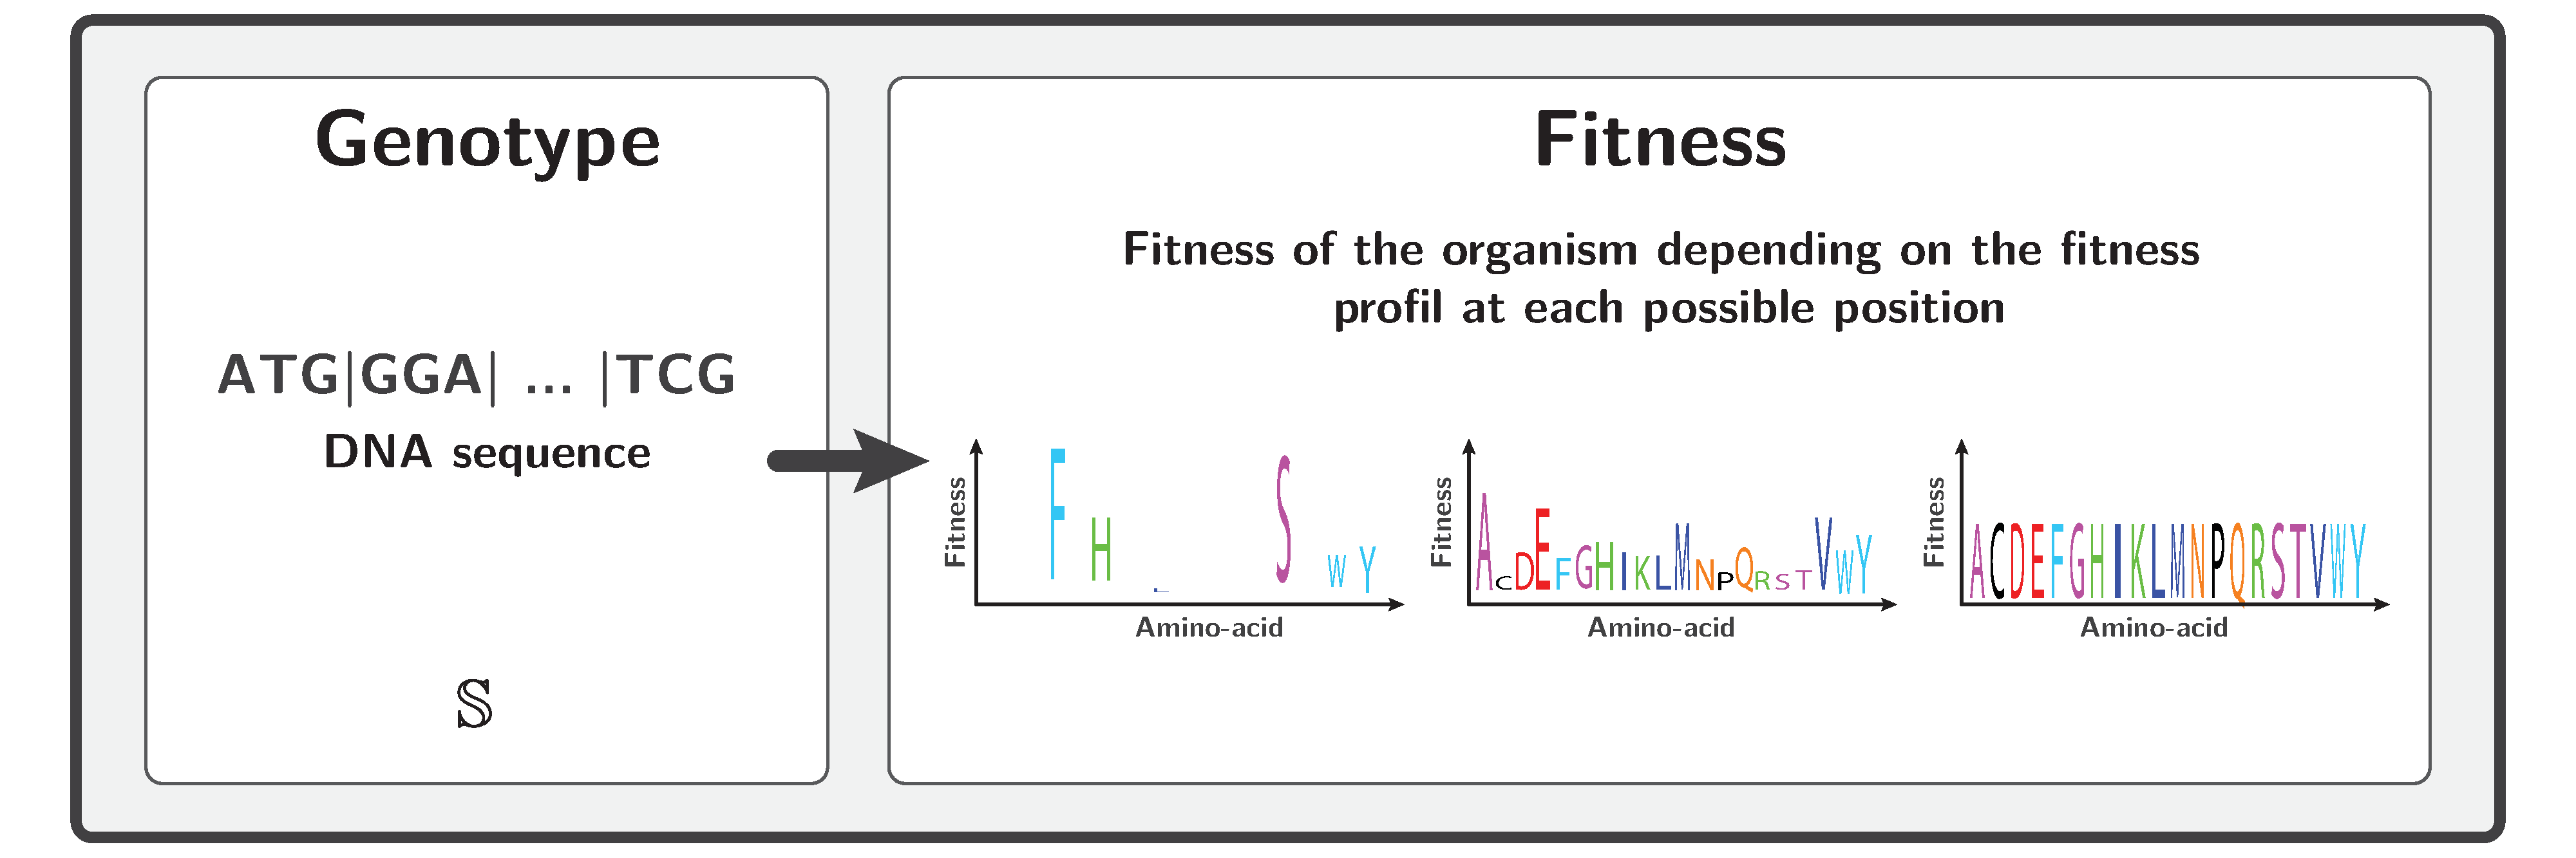
\includegraphics[width=\textwidth] {ModelSimuDiv.pdf}
\end{center}

The next change in the protein coding DNA and the time to next the event is chosen using Gillespie algorithm, according to the rates of substitution between codons:
\begin{equation}
{\submatrix_{\itoj}} = \mu_{\itoj} \dfrac{4 \Ne s \left( \mathbb{S}^{t},\mathbb{S}^{t+1}\right)}{{1 - \e^{-4 \Ne s \left( \mathbb{S}^{t},\mathbb{S}^{t+1}\right)} }}, 
\end{equation}
where ${\submatrix_{\itoj}} = \mu_{\itoj}$ in the case of synonymous substitutions.

\subsection{Wright-Fisher with polymorphism}

The evolutionary dynamics was formalized as a Wright-Fisher model with mutation, selection and drift. The population is assumed to be panmictic, with with effective population size $\Ne$ and with non-overlapping generations. 

\begin{center}
	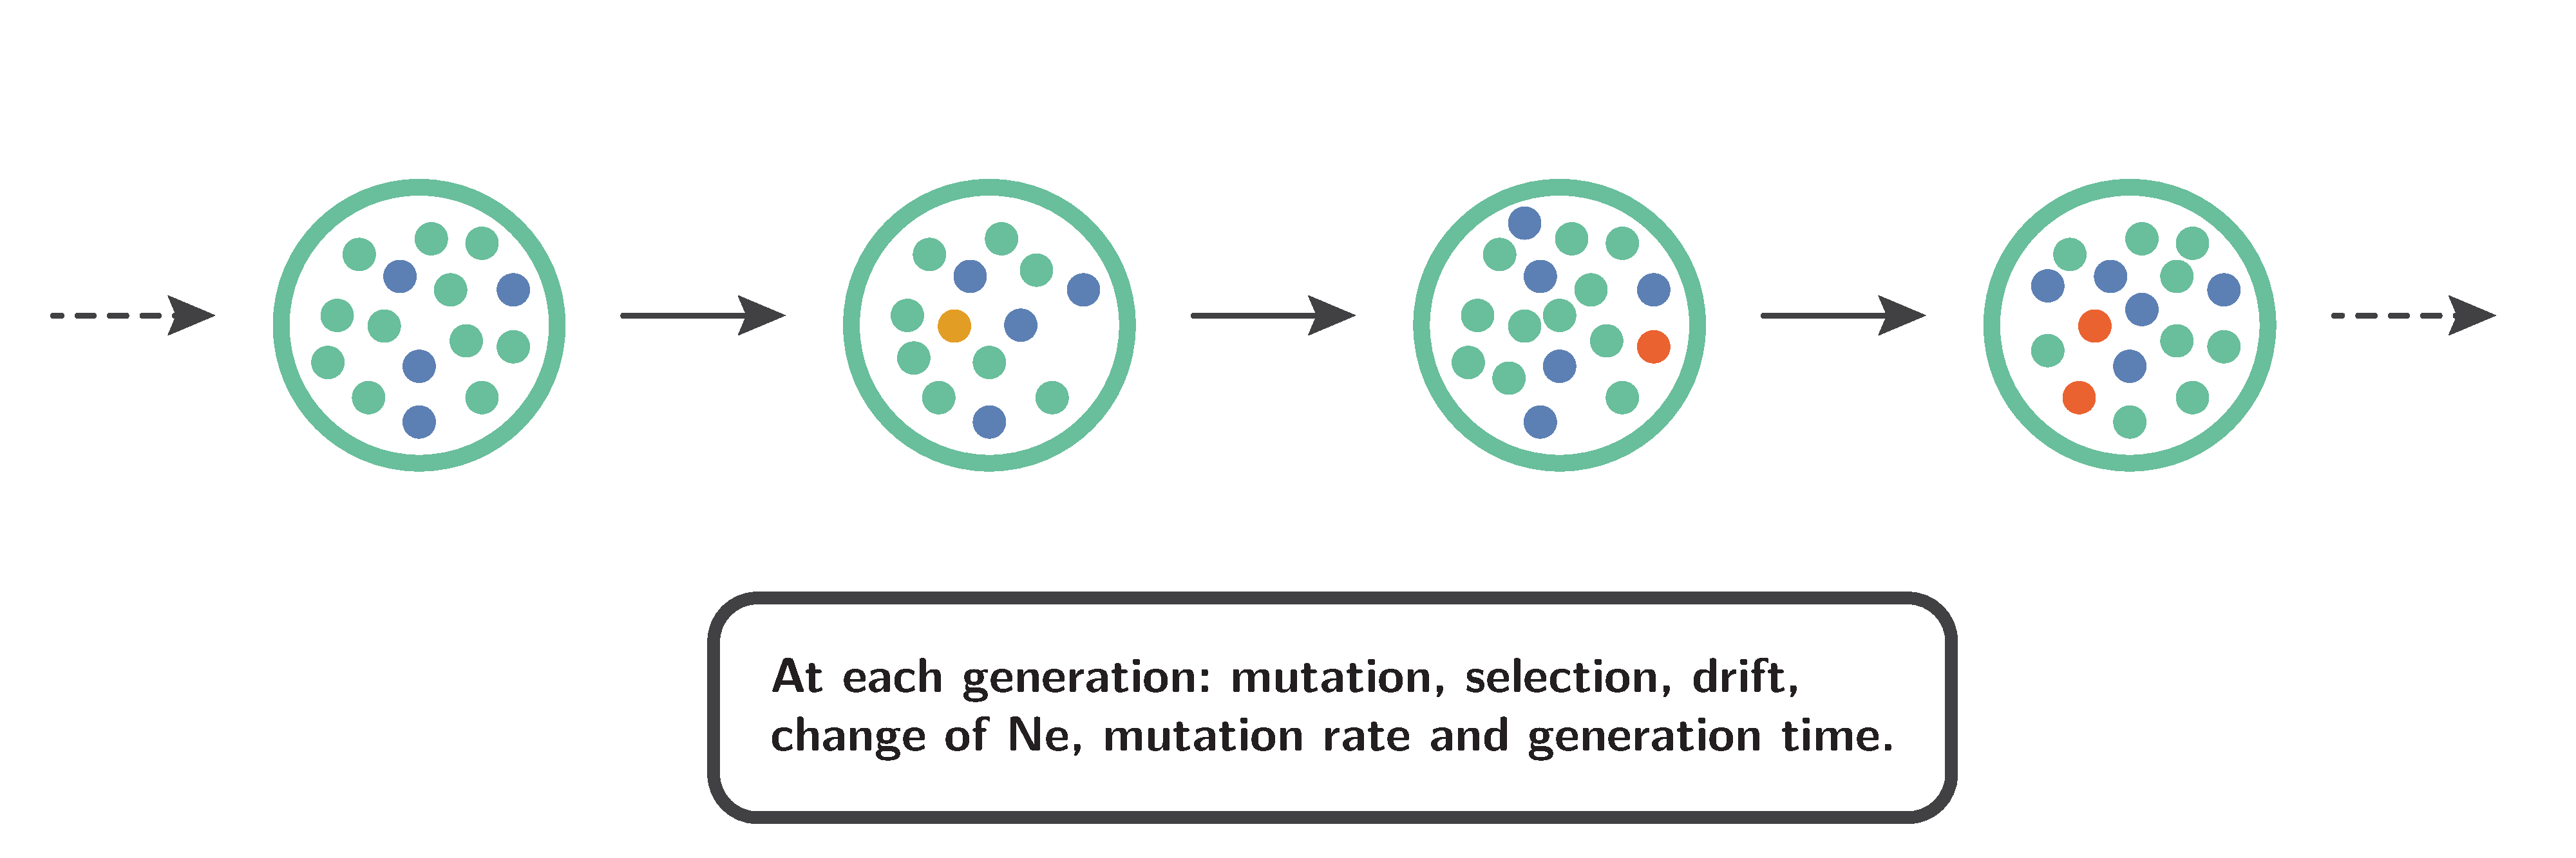
\includegraphics[width=\textwidth] {ModelSimuPoly.pdf}
\end{center}

\subsection{Fisher geometric landscape}

We simulated substitutions in a protein using an adaptation of Fisher's geometric landscape.
In the original context, the phenotype is a vector ($\phenoGeo$) in a multidimensional space, where the number of dimensions is often termed complexity.
From a phenotype, the fitness is a monotonously decreasing function of the phenotype distance to $0$.
The exact functional phenotype-fitness map depend on $2$ external parameters controlling for strength ($\alpha$) and epistasis ($\beta$).
If the phenotype-fitness map is explicit, the genotype-phenotype map is more pervasive.
Mutations are seen has displacement of the phenotype in the multidimensional space.
Beneficial mutations are moving the phenotype closer to $0$, whereas deleterious mutations are moving the phenotype further away.
In such original context, the distribution of mutational effects is not dependent on the current genotype, but this can be relaxed using a genotype-phenotype map.\\

In a protein context, the genotype-phenotype map can be defined by assigning to each of the $20$ amino-acid a vector in the multidimensional space.
Since different sites of the protein do not have the same physico-chimical properties, we can define a specific genotype-phenotype map for each position of the sequence.
Overall, the protein phenotype is computed as the sum of site-specific multidimensional vectors, obtained by accessing the amino-acid present at each site of the protein.
From a DNA sequence $\mathbb{S}^t$ after $t$ substitutions, the protein's phenotype is given by:
\begin{equation}
\phenoGeo\left(\mathbb{S}^{t}\right) = \sum_{1 \leq \site \leq \Nsite} \phenoGeo_{\site} \left(\mathbb{S}^t(\site) \right),
\end{equation}
where $\phenoGeo_{\site}$ is the genotype-phenotype map at site $\site$.\\

And the Wrightian fitness of $\mathbb{S}^t$ is : 
\begin{equation}
w\left( \phenoGeo\left(\mathbb{S}^{t}\right) \right) = e^{-\alpha \left| \phenoGeo\left(\mathbb{S}^{t}\right) \right|^{\beta}},
\end{equation}
where strength ($\alpha > 0$) and epistasis ($\beta$) are parameters of the fitness function.
\begin{center}
	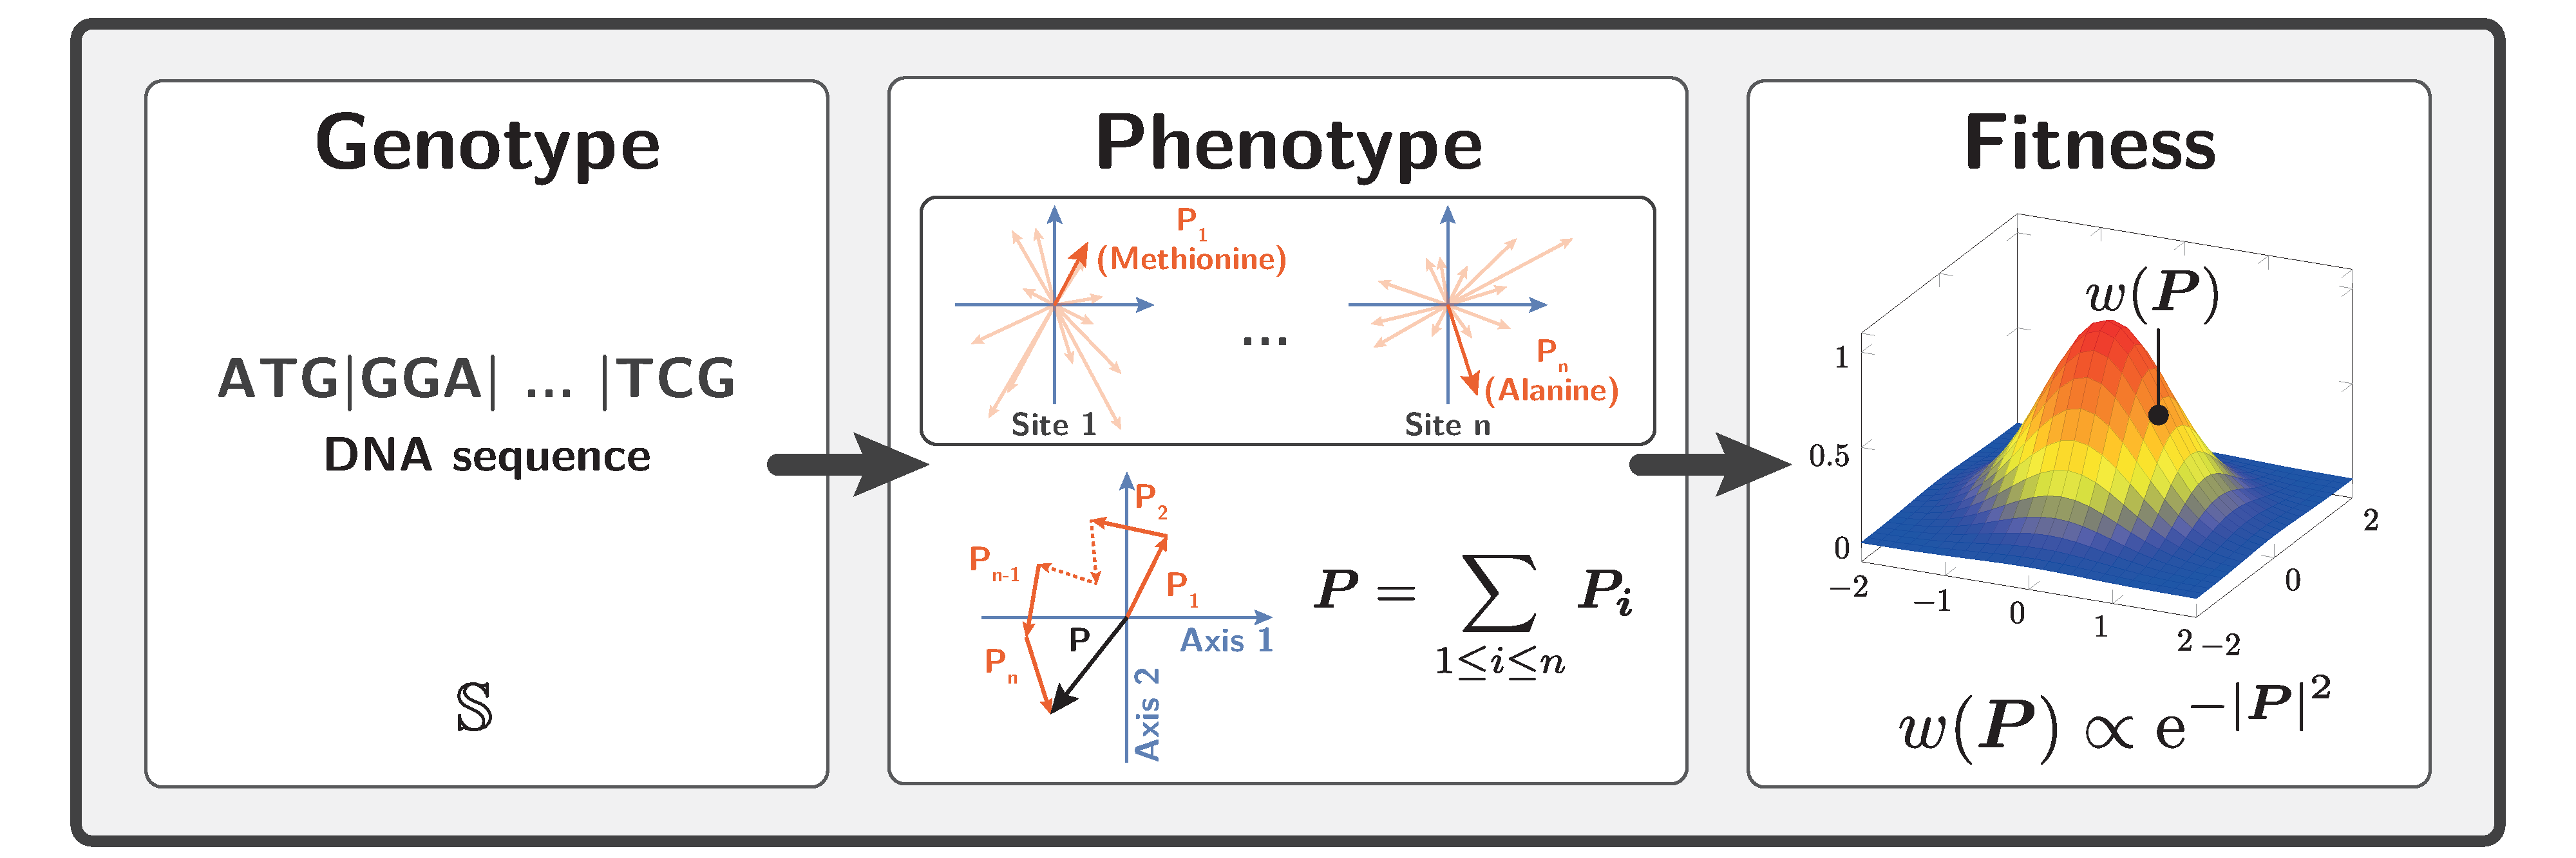
\includegraphics[width=\textwidth] {ModelSimuGeo.pdf}
\end{center}
For each possible mutant ($t+1$ substitutions), we compute $\phenoGeo\left(\mathbb{S}^{t+1}\right)$ from the updated sequence $\mathbb{S}^{t+1}$, and subsequently the selection coefficient of the mutant:
\begin{equation}
s \left( \mathbb{S}^{t},\mathbb{S}^{t+1}\right) = \dfrac{ w\left( \phenoGeo\left(\mathbb{S}^{t+1}\right) \right) - w\left( \phenoGeo\left(\mathbb{S}^{t}\right) \right)}{w\left( \phenoGeo\left(\mathbb{S}^{t}\right) \right)}.
\end{equation}
The next change in the protein coding DNA and the time to next the event is chosen using Gillespie algorithm, according to the rates of substitution between codons:
\begin{equation}
{\submatrix_{\itoj}} = \mu_{\itoj} \dfrac{4 \Ne s \left( \mathbb{S}^{t},\mathbb{S}^{t+1}\right)}{{1 - \e^{-4 \Ne s \left( \mathbb{S}^{t},\mathbb{S}^{t+1}\right)} }}, 
\end{equation}
where ${\submatrix_{\itoj}} = \mu_{\itoj}$ in the case of synonymous substitutions.

\subsection{Protein folding probability}
We simulated substitutions in the protein phosphatase ($\Nsite=300$ codon sites) as in Goldstein \& Pollock (2017).
From a DNA sequence $\mathbb{S}^t$ after $t$ substitutions, we compute the free energy of the folded state $G_{\mathrm{F}}\left(\mathbb{S}^{t}\right)$, using the $3$-dimensional structure of the folded state and pair-wise contact energies between neighboring amino-acid residues:
\begin{equation}
G_{\mathrm{F}}\left(\mathbb{S}^{t}\right) = \sum_{1 \leq \site \leq \Nsite} \sum_{r \in \mathcal{N}(\site)} I \left(\mathbb{S}^t(\site), \mathbb{S}^t(r) \right),
\end{equation}
where $I(a,b)$ is the pair-wise contact energies between amino-acid $a$ and $b$, using contact potentials estimated by Miya-zawa and Jernigan, and $\mathcal{N}(\site)$ are the neighbor residues of site $\site$ (closer than $7\angstrom$) in the $3$D structure.\\

The free energy of unfolded states $G_{\mathrm{U}}\left(\mathbb{S}^{t}\right)$ is approximated using $55$ decoy $3$D structures that supposedly represent a sample of possible unfolded states:
\begin{equation}
G_{\mathrm{U}}\left(\mathbb{S}^{t}\right) = \langle G\left(\mathbb{S}^{t}\right) \rangle - kT \ln (1.0\mathrm{E}^{160}) - \dfrac{2 \left[ \langle G\left(\mathbb{S}^{t}\right)^2 \rangle - \langle G\left(\mathbb{S}^{t}\right) \rangle^2\right] }{kT}
\end{equation}
where the average $\langle . \rangle$ runs other the $55$ decoy $3$D structures, and $k$ is the Boltzmann constant and $T$ the temperature in Kelvin.\\

From the energy of folded and unfolded states, we can compute the difference in free energy between the states:
\begin{equation}
\phenoFold\left(\mathbb{S}^{t}\right) = G_{\mathrm{F}}\left(\mathbb{S}^{t}\right) - G_{\mathrm{U}}\left(\mathbb{S}^{t}\right)
\end{equation}

Wrightian fitness is defined as the probability of our protein to be in the folded state: 
\begin{equation}
w(\phenoFold\left(\mathbb{S}^{t}\right)) = \dfrac{P_{\mathrm{F}}\left(\mathbb{S}^{t}\right)}{P_{\mathrm{F}}\left(\mathbb{S}^{t}\right) + P_{\mathrm{U}}\left(\mathbb{S}^{t}\right)} = \dfrac{e^{-\beta G_{\mathrm{F}}\left(\mathbb{S}^{t}\right) }}{e^{-\beta G_{\mathrm{F}} \left(\mathbb{S}^{t}\right) } + e^{-\beta G_{\mathrm{U}}\left(\mathbb{S}^{t}\right) }} = \dfrac{1}{1 + e^{\beta \phenoFold\left(\mathbb{S}^{t}\right) }}, 
\end{equation}
where $\beta$ is the inverse of the temperature ($\beta=1/kT$).
\begin{center}
	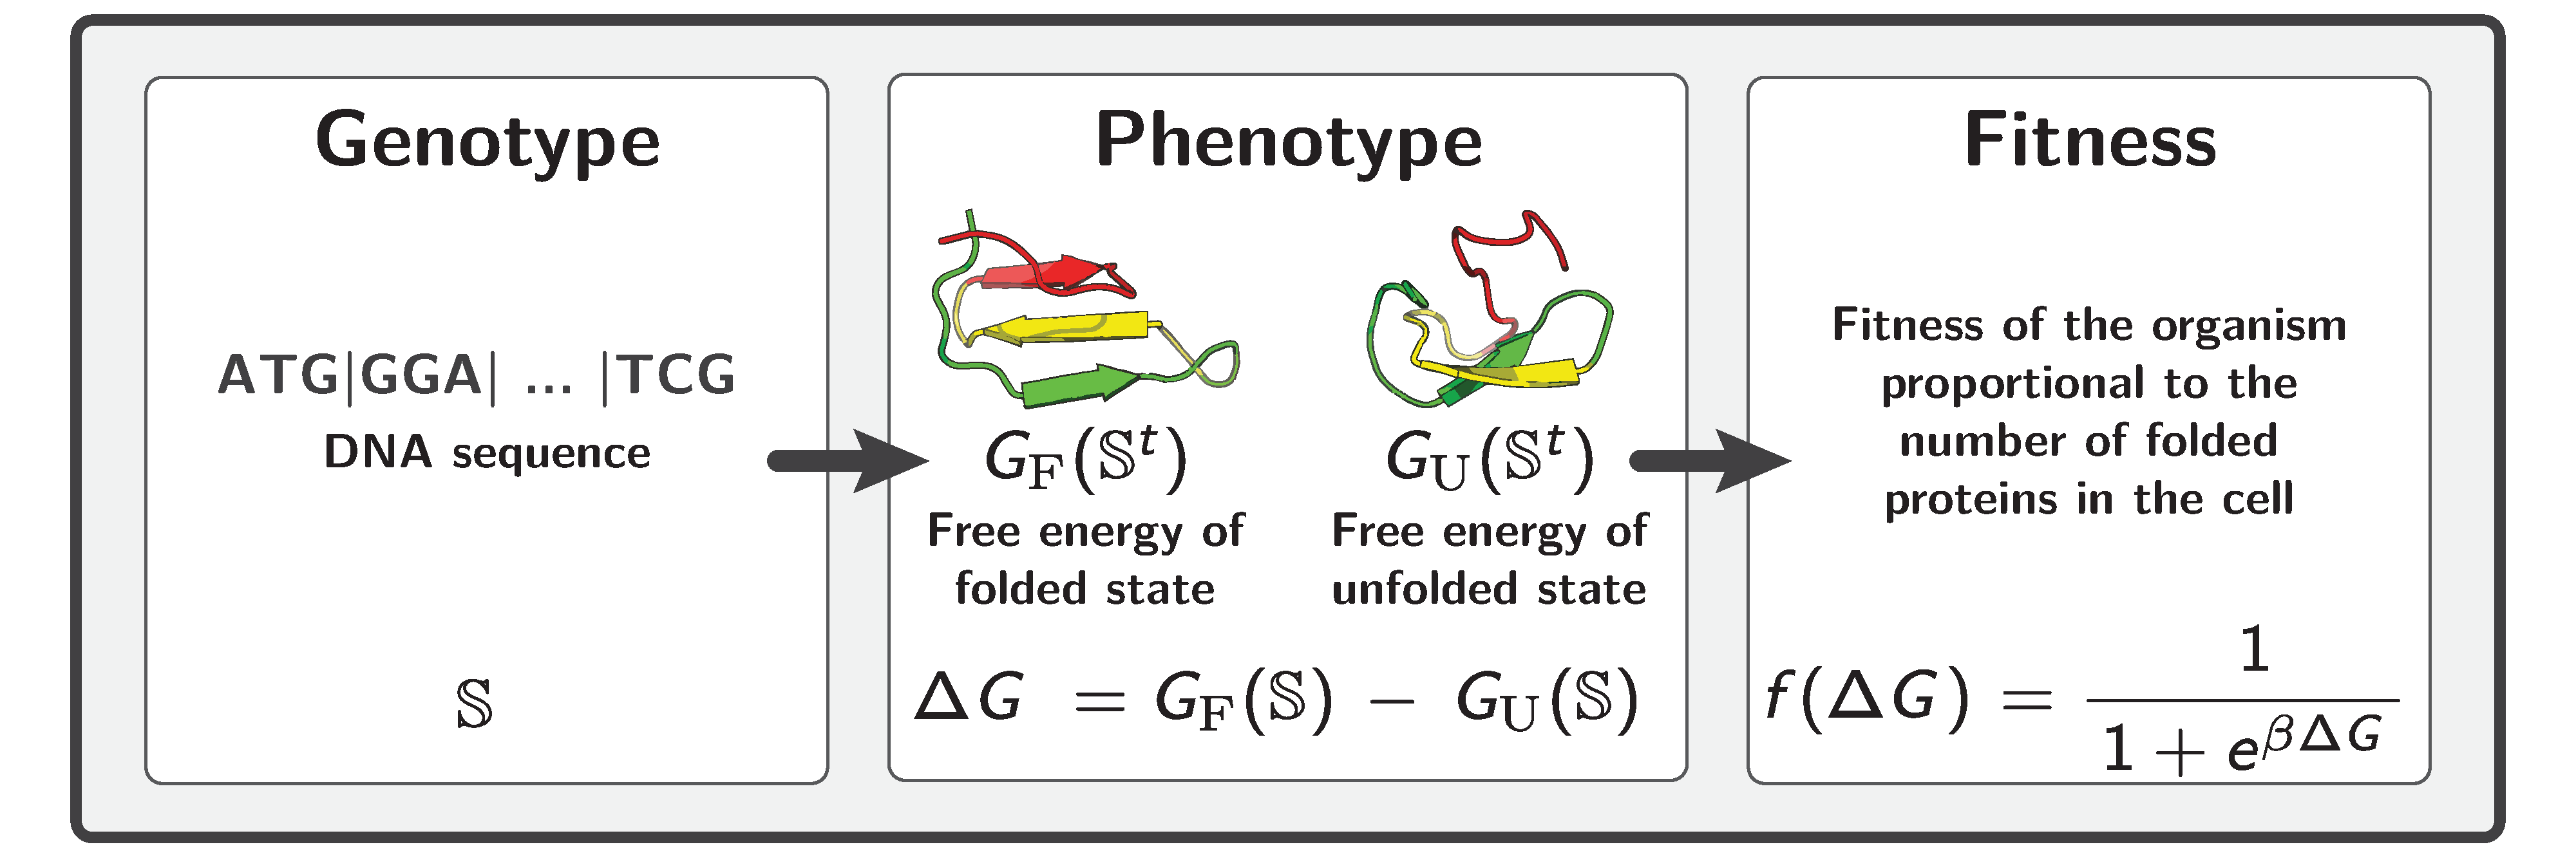
\includegraphics[width=\textwidth] {ModelSimuFold.pdf}
\end{center}
For each possible mutant ($t+1$ substitutions), we compute $\phenoFold^{t+1}$ from the updated sequence $\mathbb{S}^{t+1}$, and subsequently the selection coefficient of the mutant:
\begin{equation}
s \left( \mathbb{S}^{t},\mathbb{S}^{t+1}\right) = \dfrac{ w\left( \phenoFold\left(\mathbb{S}^{t+1}\right) \right) - w\left( \phenoFold\left(\mathbb{S}^{t}\right) \right)}{w\left( \phenoFold\left(\mathbb{S}^{t}\right) \right)}.
\end{equation}
The next change in the protein coding DNA and the time to next the event is chosen using Gillespie algorithm, according to the rates of substitution between codons:
\begin{equation}
{\submatrix_{\itoj}} = \mu_{\itoj} \dfrac{4 \Ne s \left( \mathbb{S}^{t},\mathbb{S}^{t+1}\right)}{{1 - \e^{-4 \Ne s \left( \mathbb{S}^{t},\mathbb{S}^{t+1}\right)} }}, 
\end{equation}
where ${\submatrix_{\itoj}} = \mu_{\itoj}$ in the case of synonymous substitutions.

\section{Simulated experiments}

\subsection{Independent contrasts in simulated experiment}
\begin{figure}[H]
	\centering
	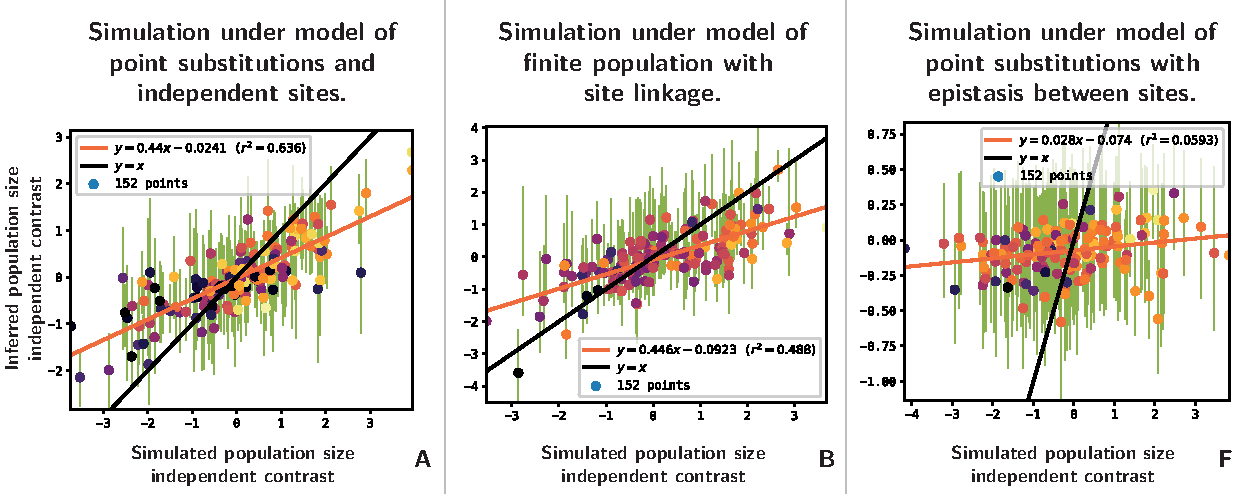
\includegraphics[width=\textwidth] {simulations_contrast.pdf}
	\caption[Inferred and simulated $\Ne$]{
		Inferred and simulated $\Ne$.
		Bottom row, independent contrast of $\Ne$ for each branch of the tree, discarding effect of phylogenetic inertia.
		Panel A, simulation accounting for long term fluctuation of $\Ne$, mutation rate per generation and generation time.
		Panel B, simulation accounting for finite population effects, site linkage and short term fluctuation of $\Ne$.
		Panel C, simulation accounting for site epistasis, thus fluctuation of the selection coefficient along the phylogeny.
	}
	\label{fig:independent}
\end{figure}

\section{Partial correlation in placental mammals}
The correlation coefficient $\rho_{\traiti, \traitj}$ give the total regression between two variable.
Partial-correlation coefficient account for the entire covariance matrix, and measure the correlation between $2$ traits, knowing the values of all the other traits: 
\begin{equation}
\rho_{\traiti, \traitj | c \in \traitInterval \setminus \{ a, b\} } = - \dfrac{\Precisionmatrix_{\traiti, \traitj}}{\sqrt{\Precisionmatrix_{\traiti, \traiti} \Precisionmatrix_{\traitj, \traitj}}}, 
\end{equation}
where the precision matrix $\PrecisionMatrix$ is the inverse of the covariance matrix:
\begin{equation}
\PrecisionMatrix = \CovarianceMatrix^{-1}
\end{equation}

\begin{table}[H]
	\centering
	\resizebox{\columnwidth}{!}{%
	\begin{tabu}{|c||c|c|c|c|c|}
		\hline
		& \specialcell{$\Ne$} & \specialcell{$\mu$} & \specialcell{Maximum\\longevity (yrs)} & \specialcell{Adult\\weight (g)} & \specialcell{Female\\maturity (days)}\\
		\hline
		\hline\specialcell{$\Ne$} & $\dots$ & $0.36^{**}$ & $-0.15$ & $0.036$ & $0.093$\\
		\hline\specialcell{$\mu$} & $0.36^{**}$ & $\dots$ & $-0.33^{**}$ & $-0.37^{**}$ & $-0.14$\\
		\hline\specialcell{Maximum longevity (yrs)} & $-0.15$ & $-0.33^{**}$ & $\dots$ & $0.25^{**}$ & $0.43^{**}$\\
		\hline\specialcell{Adult weight (g)} & $0.036$ & $-0.37^{**}$ & $0.25^{**}$ & $\dots$ & $0.27^{**}$\\
		\hline\specialcell{Female maturity (days)} & $0.093$ & $-0.14$ & $0.43^{**}$ & $0.27^{**}$ & $\dots$\\
		\hline
	\end{tabu}}
	\caption[Partial correlation coefficient matrix]{
	Partial correlation coefficient between effective population size~($\Ne$), mutation rate per site per unit of time~($\mu$), and life-history traits (Maximum longevity, adult weight and female maturity) were computed in placental mammals.
	Asterisks indicate strength of support ($\smash{^{*}} pp > 0.95$, $\smash{^{**}} pp > 0.975$).}
\end{table}

\section{Fitness profile entropy}
For a category $\cat$, the Shannon entropy ($\Omega$) of the fitness profile is defined as:
\begin{equation}
\Omega \left( \Base\catexp \right) = - \sum_{\aSetAa} \base\catexp_{\aminoacid} \log \left( \base\catexp_{\aminoacid} \right)
\end{equation}
The Shannon entropy  measures the flatness of the fitness profile, with a value of $0$ corresponding to a single peak fitness landscape (only one amino-acid is present), and a value of $log(20)\simeq3$ corresponding to a neutral landscape, where each amino-acid has the same fitness.

The Shannon entropy can be averaged out as:
\begin{equation}
\langle \Omega \left( \Fit \right) \rangle = \dfrac{1}{\Ncat}\sum_{\Setcat} \Omega \left( \Base\catexp \right)
\end{equation}
The average Shannon entropy was obtained in a context of constant $\Ne$ along the tree, and compared with the experiment where $\Ne$ is allowed to vary according to a log-Brownian process.
\begin{table}[H]
	\centering
	\begin{tabu}{|c|c|c|}
		\hline
		$\langle \Omega \left( \Fit \right) \rangle$ & \specialcell{\textbf{Constant} $\Ne$} & \specialcell{\textbf{log-Brownian} $\Ne$} \\
		\hline
		\hline\specialcell{Placental mammals, replicate $1$, chain $1$} & $1.34 \pm 0.09$ & $1.24 \pm 0.09$ \\
		\hline\specialcell{Placental mammals, replicate $1$, chain $2$} & $1.33 \pm 0.08$ & $1.27 \pm 0.10$ \\
		\hline\specialcell{Placental mammals, replicate $2$, chain $1$} & $1.40 \pm 0.06$ & $1.31 \pm 0.09$ \\
		\hline\specialcell{Placental mammals, replicate $2$, chain $2$} & $1.42 \pm 0.07$ & $1.28 \pm 0.11$ \\
		\hline\specialcell{Placental mammals, replicate $3$, chain $1$} & $1.23 \pm 0.08$ & $1.25 \pm 0.12$ \\
		\hline\specialcell{Placental mammals, replicate $3$, chain $2$} & $1.25 \pm 0.09$ & $1.24 \pm 0.10$ \\
		\hline
	\end{tabu}
\end{table}

\section{Likelihood of divergence data}
The probability of transition between codons for a given branch $\branch$ and site $\site$ is:
\begin{equation}
\Probmatrix\branchsiteexp = \e^{\branchlength\branchexp \Submatrix\branchsiteexp}
\end{equation}
The likelihood of the data $\Data$ can be computed using the pruning algorithm:
\begin{equation}
p\left(\Data\siteexp|\Subequi^{\treerootexp}, \Probmatrix\branchsiteexp \right) = \sum_{\iSetCodon } \subequi_{\ci}^{\treerootsiteexp} \pruning\siteexp_{\treeroot} \left( \ci, \Probmatrix\branchsiteexp \right)
\end{equation}
where $\pruning_{\node} \left( \ci \right)$ is computed recursively from the $2$  descendant children $\node_{1}$ and $\node_{2}$ of an internal node $\node$:
\begin{equation}
\pruning\siteexp_{\node} \left( \ci \right) = \left[ \sum_{\jSetCodon} \probmatrix^{(\branchnode\left(\node_{1}\right), \site)}_{\itoj} \pruning\siteexp_{\node_{1}} \left( \cj, \Probmatrix\branchsiteexp \right) \right] \cdot \left[ \sum_{\jSetCodon} \probmatrix^{(\branchnode\left(\node_{1}\right), \site)}_{\itoj} \pruning\siteexp_{\node_{2}} \left( \cj, \Probmatrix\branchsiteexp \right) \right]
\end{equation}
And if the node $\node$ is a node with no descendant, meaning $\Settaxon$:
\begin{equation}
\pruning\siteexp_{\node}\left( \ci, \Probmatrix\branchsiteexp \right) =
\begin{dcases}
1, & \text{if }\Data\taxonsiteexp =  \ci \\
0, & \text{otherwise.}
\end{dcases}
\end{equation}

\section{Sufficient statistics}
A sequence of length $\Nsite$ evolves by point substitutions, according to a random process defined by the substitution matrices $\Submatrix\branchsiteexp$, over a phylogenetic tree.
A realization of the random process along a branch $\branch$, and at a particular site $\site$ results in a detailed substitution history, which will be denoted by $\subhistory\branchsiteexp$.

\subsubsection{Path sufficient statistics}
All sites owning to the same category of fitness profile share the same substitution rate matrix.
Hence, $\subhistory\branchsiteexp$ can be gathered across all sites owing to a specific category $\cat$, denoted $\subhistory\branchexp$.
If we express the probability of the substitution mapping ($\subhistory\branchcatexp$) as a function of the codon substitution process for this category $\cat$, we get the following expression:
\begin{equation}
\label{eq:PathSuffStat}
p(\subhistory\branchcatexp | \branchlength\branchexp, \Submatrix\branchcatexp) \propto \prod_{\iSetCodon} \left[\subequi_{\ci}\branchcatexp\right]^{n_{\ci}\branchcatexp} \prod_{ \ijSetCodon} \left[\submatrix\branchcatexp_{\itoj}\right]^{m_{\ci, \cj}\branchcatexp} \prod_{\iSetCodon} \e^{- \left|  \submatrix\branchcatexp_{\ci, \ci}\right| a_{\ci}\branchcatexp}
\end{equation}
where we define the sufficient statistics:
\begin{itemize}
	\setlength\itemsep{-0.25em}
	\item $m_{\ci, \cj}\branchcatexp$ is the total number of substitutions from codon $\ci$ to codon $\cj$
	\item $n_{\ci}\branchcatexp$ is the number of sites starting with codon $\ci$ at the tip of the branch.
	\item $a_{\ci}\branchcatexp$ is the total waiting time in codon $\ci$.
\end{itemize}
Once these sufficient statistics have been computed, the parameters of the substitution matrix $\Submatrix\branchcatexp$ can be resampled conditional on $\subhistory\branchcatexp$, 
using equation~\ref{eq:PathSuffStat} each time the likelihood needs to be recomputed. This leads to relatively fast MCMC strategy.
\subsubsection{Length sufficient statistics}
$\subhistory\branchsiteexp$ can also be gathered across all sites along a specific branch, giving $\subhistory\branchexp$.
Then the probability of the substitution history given the branch lengths ($\branchlength\branchexp = \mu\branchexp \branchtime\branchexp$), take a very simple form:
\begin{equation}
\label{eq:LengthSuffStat}
p(\subhistory\branchexp | L\branchexp) \propto \left[ L\branchexp\right]^{u\branchexp} \e^{- r\branchexp L\branchexp}
\end{equation}
where we define the sufficient statistics:
\begin{itemize}
	\setlength\itemsep{-0.25em}
	\item $u\branchexp$ is the total number of substitutions over branch $\branch$, summed over all sites.
	\item $r\branchexp$ is the mean rate away from current codon state (averaged over the entire substitution history).
\end{itemize}
Thus, formally, the probability of the substitution mapping can be summarized by saying that the total number of substitutions along a given branch over all sites, $u\branchexp$, is Poisson distributed, of mean $r\branchexp L\branchexp$.

\subsubsection{Scatter sufficient statistics}
From the independent contrast $\contrast\branchexp$ of the Brownian process $\Brownian\nodeexp$, we can define the $2 \times 2$  scatter sufficient statistic matrix, $\Scattermatrix$ as:
\begin{equation}
\Scattermatrix = \sum_{b=1}^{\Nbranch} \contrast\branchexp \cdot \left[\contrast\branchexp\right]^{\mathrm{T}}
\end{equation}
By Bayes theorem, the posterior on $\Sigma$, conditional on a particular realization of $\brownian$ (and thus of $\contrast$) is an invert Wishart distribution, of parameter $\covariancekappa \Identitymatrix + \Scattermatrix$ and with $\Nbranch + 3$ degrees of freedom.
\begin{equation}
\CovarianceMatrix  \sim \mathrm{Wishart}^{-1}\left( \covariancekappa \Identitymatrix + \Scattermatrix, \Nbranch + 3\right)
\end{equation}
This invert Wishart distribution can be obtained by sampling $\Nbranch + 3$ independent and identically distributed multivariate normal random variables $\Multivariate\indiceexp$ defined by
\begin{equation}
\Multivariate\indiceexp \sim \mathcal{N} \left( \bm{0}, \left[\covariancekappa \Identitymatrix + \Scattermatrix\right]^{-1} \right).
\end{equation}
And from these multivariate samples, $\CovarianceMatrix$ is Gibbs sampled as:
\begin{equation}
\CovarianceMatrix = \left( \sum_{k=1}^{\Nbranch + 3} \Multivariate\indiceexp \cdot \left[\Multivariate\indiceexp \right] ^{\mathrm{T}} \right)^{-1}
\end{equation}
